\documentclass{article}
\usepackage{fullpage,graphicx}
\usepackage{amsmath,amsfonts,amsthm,amssymb,multirow}
\usepackage{algorithmic,comment,url}
\usepackage{tikz}
\usetikzlibrary{decorations.pathreplacing, shapes,positioning}
\usepackage[ruled,vlined,commentsnumbered,titlenotnumbered]{algorithm2e}
\newcommand{\expecting}[1]{\noindent{[\textbf{We are expecting:} \em #1\em]}}
\newcommand{\hint}[1]{\noindent{[\textbf{HINT:} \em #1 \em]}}
\newcommand{\pts}[1]{\textbf{(#1 pt.)}}


\begin{document}
\noindent
CS 161 \hfill \textbf{Problem Set 5} \newline 
{Winter 2019} \hfill \textbf{Due:} Friday, March 1, 2019, at 3pm on Gradescope

\noindent
\rule{\linewidth}{0.4pt}
\noindent
\section*{Exercises}
Please do the exercises on your own.

\noindent
\rule{\linewidth}{0.4pt}
\begin{enumerate}

\item \pts{6} Consider the following directed graph:

\begin{center}
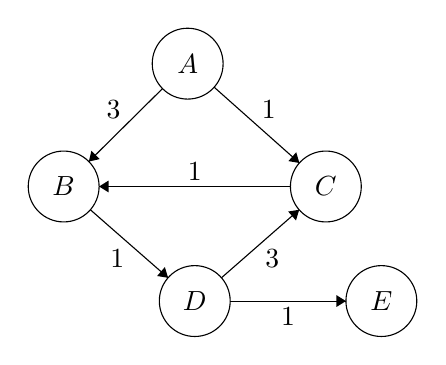
\begin{tikzpicture}[scale=0.15]
\tikzstyle{every node}+=[inner sep=0pt]
\draw [black] (38,-18) circle (3);
\draw (38,-18) node {$A$};
\draw [black] (27.5,-28.4) circle (3);
\draw (27.5,-28.4) node {$B$};
\draw [black] (49.7,-28.4) circle (3);
\draw (49.7,-28.4) node {$C$};
\draw [black] (38.6,-38.1) circle (3);
\draw (38.6,-38.1) node {$D$};
\draw [black] (54.4,-38.1) circle (3);
\draw (54.4,-38.1) node {$E$};
\draw [black] (35.87,-20.11) -- (29.63,-26.29);
\fill [black] (29.63,-26.29) -- (30.55,-26.08) -- (29.85,-25.37);
\draw (31.73,-22.72) node [above] {$3$};
\draw [black] (40.24,-19.99) -- (47.46,-26.41);
\fill [black] (47.46,-26.41) -- (47.19,-25.5) -- (46.53,-26.25);
\draw (44.86,-22.71) node [above] {$1$};
\draw [black] (46.7,-28.4) -- (30.5,-28.4);
\fill [black] (30.5,-28.4) -- (31.3,-28.9) -- (31.3,-27.9);
\draw (38.6,-27.9) node [above] {$1$};
\draw [black] (29.76,-30.37) -- (36.34,-36.13);
\fill [black] (36.34,-36.13) -- (36.07,-35.22) -- (35.41,-35.98);
\draw (32.04,-33.74) node [below] {$1$};
\draw [black] (40.86,-36.13) -- (47.44,-30.37);
\fill [black] (47.44,-30.37) -- (46.51,-30.52) -- (47.17,-31.28);
\draw (45.16,-33.74) node [below] {$3$};
\draw [black] (41.6,-38.1) -- (51.4,-38.1);
\fill [black] (51.4,-38.1) -- (50.6,-37.6) -- (50.6,-38.6);
\draw (46.5,-38.6) node [below] {$1$};
\end{tikzpicture}
\end{center}

For the following parts you might want to use this website, which allows you to draw directed graphs in \LaTeX: \url{http://madebyevan.com/fsm/}.  (Note: On a Mac, fn+Delete will delete nodes or edges).  It is also fine to include an image created in your favorite drawing program, or a photo/scan of a hand-drawn graph.

\begin{enumerate}
\item \pts{2} Draw the DFS tree for this graph, starting from node A.  Assume that DFS traverses nodes in alphabetical order.  (That is, if it could go to either $B$ or $C$, it will always choose $B$ first).

\item \pts{2} Draw the BFS tree for this graph, starting from node A.  Assume that BFS traverses nodes in alphabetical order.  

\item \pts{2} Draw the ``Dijkstra's algorithm tree'' for this graph, starting from node A.  Assume that Dijkstra's algorithm breaks ties in alphabetical order. 
\end{enumerate}

\expecting{Pictures of your trees.  No further explanation is required.}

\newpage
\item \pts{4} Consider the following directed acyclic graph (DAG):
\begin{center}
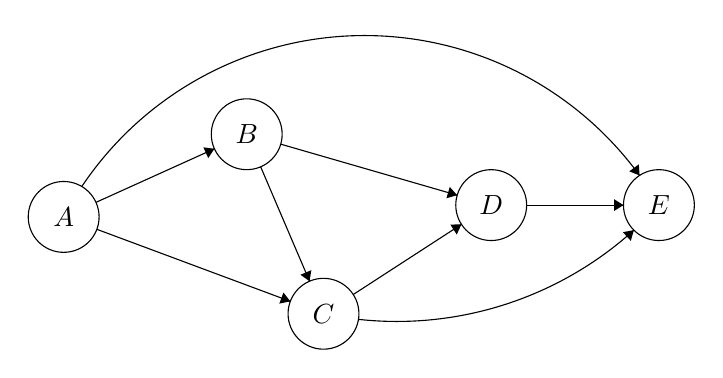
\begin{tikzpicture}[scale=0.15]
\tikzstyle{every node}+=[inner sep=0pt]
\draw [black] (18.2,-24.6) circle (3);
\draw (18.2,-24.6) node {$A$};
\draw [black] (33.7,-17.6) circle (3);
\draw (33.7,-17.6) node {$B$};
\draw [black] (40.2,-32.8) circle (3);
\draw (40.2,-32.8) node {$C$};
\draw [black] (54.4,-23.6) circle (3);
\draw (54.4,-23.6) node {$D$};
\draw [black] (68.6,-23.6) circle (3);
\draw (68.6,-23.6) node {$E$};
\draw [black] (57.4,-23.6) -- (65.6,-23.6);
\fill [black] (65.6,-23.6) -- (64.8,-23.1) -- (64.8,-24.1);
\draw [black] (20.93,-23.37) -- (30.97,-18.83);
\fill [black] (30.97,-18.83) -- (30.03,-18.71) -- (30.44,-19.62);
\draw [black] (34.88,-20.36) -- (39.02,-30.04);
\fill [black] (39.02,-30.04) -- (39.17,-29.11) -- (38.25,-29.5);
\draw [black] (42.72,-31.17) -- (51.88,-25.23);
\fill [black] (51.88,-25.23) -- (50.94,-25.25) -- (51.48,-26.09);
\draw [black] (21.01,-25.65) -- (37.39,-31.75);
\fill [black] (37.39,-31.75) -- (36.81,-31) -- (36.46,-31.94);
\draw [black] (36.58,-18.44) -- (51.52,-22.76);
\fill [black] (51.52,-22.76) -- (50.89,-22.06) -- (50.61,-23.02);
\draw [black] (19.736,-22.025) arc (146.19641:36.07693:28.811);
\fill [black] (66.96,-21.09) -- (66.9,-20.15) -- (66.09,-20.74);
\draw [black] (66.48,-25.721) arc (-47.8655:-96.2357:29.916);
\fill [black] (66.48,-25.72) -- (65.55,-25.89) -- (66.22,-26.63);
\end{tikzpicture}
\end{center}
In class,
we saw how to use DFS to find a topological ordering of the the vertices; in the graph above, the unique topological ordering is $A,B,C,D,E$.  We saw an example where we happened to start DFS from the first vertex in the topological order.  In this exercise we'll see what happens when we start at a different vertex.  Recall that when you run DFS, if it has reached everything it can but hasn't yet explored the graph, it will start again at an unexplored vertex.

\begin{enumerate}
\item Run DFS starting at vertex $C$, breaking any ties by alphabetical order.\footnote{For example, if DFS has a choice between $B$ or $C$, it will always choose $B$.  This includes when DFS is starting a new tree in the DFS forest.} 
\begin{enumerate}
\item
What do you get when you order the vertices by \textbf{ascending} start time?
\item What do you get when you order the vertices by \textbf{descending} finish time?
\end{enumerate}
\item Run DFS starting at vertex $C$, breaking any ties by \textbf{reverse} alphabetical order.\footnote{For example, when DFS has a choice between $B$ or $C$, it will always choose $C$. This includes when DFS is starting a new tree in the DFS forest.} 
\begin{enumerate}
\item What do you get when you order the vertices by \textbf{ascending} start time?
\item What do you get when you order the vertices by \textbf{descending} finish time?
\end{enumerate}
\end{enumerate}

\expecting{For all four questions, an ordering of vertices. No justification is required.}



\newpage
\item \pts{6}
In class, we saw pseudocode for Dijkstra's algorithm which returned shortest distances but not shortest paths.  In this exercise we'll see how to adapt it to return shortest paths.  One way to do that is shown in the pseudocode below: 

\begin{verbatim}
Dijkstra_st_path(G, s, t):
    for all v in V, set d[v] = Infinity
    for all v in V, set p[v] = None 
    // we will use the information p[v] to reconstruct the path at the end.
    d[s] = 0
    F = V
    D = []  // D is the list of "done" vertices
    while F isn't empty:  
        x = a vertex v in F so that d[v] is minimal
        for y in x.outgoing_neighbors:
            d[y] = min( d[y], d[x] + weight(x,y) )
            if d[y] was changed in the previous line, set p[y] = x
        F.remove(x)
        D.add(x)
        
    // use the information in p to reconstruct the shortest path:
    path = [t]
    current = t
    while current != s:
        current = p[current]
        add current to the front of the path
    return path, d[t]
\end{verbatim}

Step through \texttt{Dijkstra\_st\_path}$(G,s,t)$ on the graph $G$ shown below.
        Complete the table below (on the next page) to show what the arrays \texttt{d} and \texttt{p} are at each step of the algorithm, and indicate what path is returned and what its cost is.   If it is helpful, the \LaTeX code for the table is reproduced at the end of the PSET.

\begin{center}
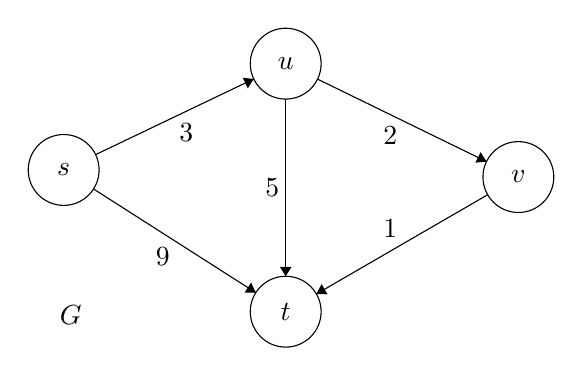
\begin{tikzpicture}[scale=0.15]
\tikzstyle{every node}+=[inner sep=0pt]
\draw [black] (16.8,-26.3) circle (3);
\draw (16.8,-26.3) node {$s$};
\draw [black] (35.6,-17.3) circle (3);
\draw (35.6,-17.3) node {$u$};
\draw [black] (55.3,-26.9) circle (3);
\draw (55.3,-26.9) node {$v$};
\draw [black] (35.6,-38.3) circle (3);
\draw (35.6,-38.3) node {$t$};
\draw [black] (19.51,-25) -- (32.89,-18.6);
\fill [black] (32.89,-18.6) -- (31.96,-18.49) -- (32.39,-19.39);
\draw (27.19,-22.31) node [below] {$3$};
\draw [black] (38.3,-18.61) -- (52.6,-25.59);
\fill [black] (52.6,-25.59) -- (52.1,-24.79) -- (51.66,-25.68);
\draw (44.46,-22.61) node [below] {$2$};
\draw [black] (52.7,-28.4) -- (38.2,-36.8);
\fill [black] (38.2,-36.8) -- (39.14,-36.83) -- (38.64,-35.96);
\draw (44.45,-32.1) node [above] {$1$};
\draw [black] (19.33,-27.91) -- (33.07,-36.69);
\fill [black] (33.07,-36.69) -- (32.67,-35.83) -- (32.13,-36.68);
\draw (25.2,-32.8) node [below] {$9$};
\draw [black] (35.6,-20.3) -- (35.6,-35.3);
\fill [black] (35.6,-35.3) -- (36.1,-34.5) -- (35.1,-34.5);
\draw (35.1,-27.8) node [left] {$5$};
\draw (17.4,-38.6) node {$G$};
\end{tikzpicture}
\end{center}


\expecting{The following things:
\begin{itemize}
\item The table below filled out
\item The shortest path and its cost that the algorithm returns. 
\end{itemize}
No justification is required.}

%%%%%%%%%%%%%%%%%%%  TABLE:  Fill in your answers between the & symbols below if you wish to take this LaTeX code for your solution.

\begin{center}
\def\arraystretch{1.5}
\newcommand{\td}{\texttt{d}}
\newcommand{\tp}{\texttt{p}}
\begin{tabular}{|p{6cm}||c|c|c|c||c|c|c|c|}
\hline
& \td[$s$] & \td[$u$] & \td[$v$] & \td[$t$] & \tp[$s$] & \tp[$u$] & \tp[$v$] & \tp[$t$] \\
\hline
When entering the first while loop for the first time, the state is:&
0 & $\infty$ & $\infty$ & $\infty$ & None & None & None & None \\
\hline
Immediately after the first element of $D$ is added, the state is: &
0 & $3$ & $\infty$ & $9$ & None & s & None & s \\
 \hline
Immediately after the second element of $D$ is added, the state is: &
 & & & & & & & \\
 \hline
Immediately after the third element of $D$ is added, the state is: &
 & & & & & & & \\
 \hline
Immediately after the fourth element of $D$ is added, the state is: &
 & & & & & & & \\
 \hline
\end{tabular}
\end{center}

%%%%%%%%%%  END TABLE %%%%%%%%%%%%%



\end{enumerate}
\newpage
\noindent
\rule{\linewidth}{0.4pt}
\section*{Problems}

You may talk with your fellow CS161-ers about the problems.  However:
\begin{itemize}
	\item Try the problems on your own \em before \em collaborating.
	\item Write up your answers yourself, in your own words.   You should never share your typed-up solutions with your collaborators.
	\item If you collaborated, list the names of the students you collaborated with at the beginning of each problem.
\end{itemize}

\noindent
\rule{\linewidth}{0.4pt}


\begin{enumerate}
\setcounter{enumi}{3}

\item\pts{8} (\textbf{Wake up, Sheeple!}) You arrive on an island with $n$ sheep.  The sheep have developed a pretty sophisticated society, and have a social media platform called Baaaahtter (it's like Twitter but for sheep\footnote{Also my new start-up idea}).  Some sheep follow other sheep on this platform.  Being sheep, they believe and repeat anything that they hear.  That is, they will re-post anything that any sheep they are following said.  
We can represent this by a graph, where $(a) \to (b)$ means that $(b)$ will re-post anything that $(a)$ posted.  For example, if the social dynamics on the island were:
\begin{center}
\begin{tikzpicture}[xscale=2]
\node(a) at (0,0) {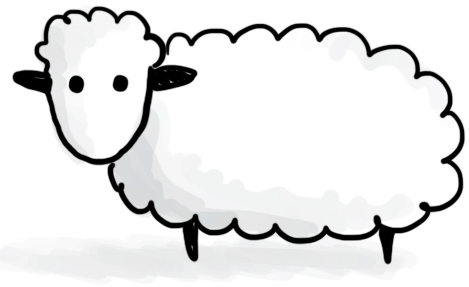
\includegraphics[width=2cm]{sheep}};
\node at (0,-1) {Shifra the sheep};
\node(b) at (2,2) {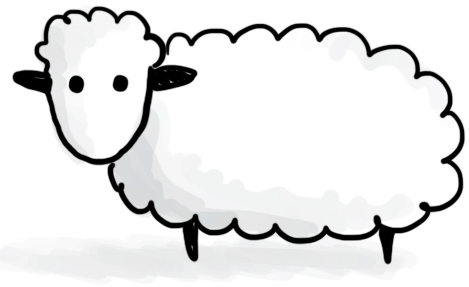
\includegraphics[width=2cm]{sheep}};
\node(bb) at (2,1) {Shakira the sheep};
\node(c) at (2,-2) {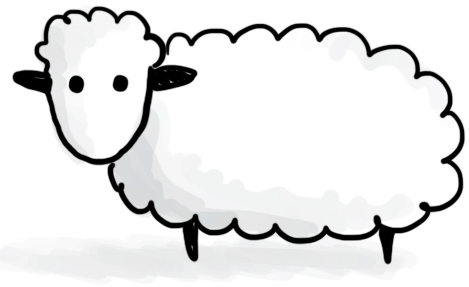
\includegraphics[width=2cm]{sheep}};
\node at (2,-3) {Sugar the sheep};
\node(d) at (4,0) {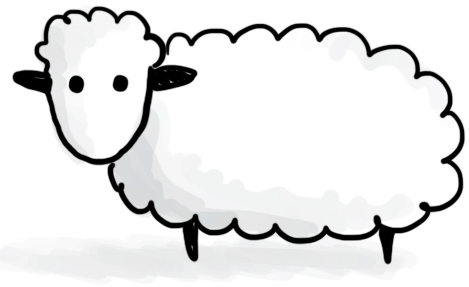
\includegraphics[width=2cm]{sheep}};
\node at (4,-1) {Sherman the sheep};
\draw[thick,->] (a) to (b);
\draw[thick,->] (b) to[bend right] (a);
\draw[thick,->] (a) to (c);
\draw[thick,->] (bb) to (c);
\draw[thick,->] (c) to (d);
\end{tikzpicture}
\end{center}
then Sherman the Sheep follows Sugar the Sheep, and Sugar follows both Shakira and Shifra, and so on.
This means that Sherman will re-post anything that Sugar posts, Sugar will re-post anything by Shifra and Shikira, and so on.
(If there is a cycle then each sheep will only re-post a post once).

For the parts below, let $G$ denote this directed, unweighted graph on the $n$ sheep.  Let $m$ denote the number of edges in $G$.

\begin{enumerate}
\item
\pts{2} Call a sheep an \textbf{influencer} if anything that they post eventually gets re-posted by every other sheep on the island.  In the example above, both Shifra and Shakira are influencers.

Prove that all influencers are in the same strongly connected component of $G$, and every sheep in that component is an influencer.

\expecting{A short but rigorous proof.}

\item \pts{4} Suppose that there is at least one influencer.  Give an algorithm that runs in time $O(n + m)$ and finds an influencer.  You may use any algorithm we have seen in class as a subroutine.

\expecting{The following things:
\begin{itemize}
\item Pseudocode or a very clear English description of your algorithm
\item an informal justification that your algorithm is correct
\item an informal justification that the running time is $O(n+m)$
\end{itemize}  You may use any statement we have proved in class without re-proving it.}

\item \pts{2} Suppose that you don't know whether or not there is an influencer.  Give an algorithm that runs in time $O(n + m)$ and either returns an influencer or returns \texttt{no influencer.}  You may use any algorithm we have seen from class as a subroutine, and you may also use your algorithm from part (b) as a subroutine.

\expecting{The following things:
\begin{itemize}
\item Pseudocode or a very clear English description of your algorithm
\item an informal justification that your algorithm is correct
\item an informal justification that the running time is $O(n+m)$
\end{itemize}  You may use any statement we have proved in class without re-proving it.}
\end{enumerate}


\vspace{2cm}
\item 
\pts{5}
(\textbf{Dijkstra with negative edges}) 
For both of the questions below, suppose that $G$ is a connected, directed, weighted graph, which may have negative edge weights, containing vertices $s$ and $t$, and refer to the pseudocode for \texttt{Dijkstra\_st\_path} from Exercise 3.  Suppose that there \em is \em some path from $s$ to $t$ in $G$. 
\begin{enumerate}
    	\item \pts{2} Give an example of a graph where there is a path from $s$ to $t$, but no shortest path from $s$ to $t$.  (Note that in a directed graph, a \em path \em must follow the direction of the edges; recall that a \em shortest path \em is one which minimizes the sum of the edge weights along that path).

\expecting{\begin{itemize}
\item A small example (at most $5$ vertices) 
\item An explanation of why there is no shortest path from $s$ to $t$.
\end{itemize}}

	\item \pts{3} Give an example of a graph where there \em is \em a shortest path from $s$ to $t$, 

but \texttt{Dijkstra\_st\_path}$(G,s,t)$ does not return one.  

\expecting{\begin{itemize}
\item A small example (at most $5$ vertices) 
\item An explanation of what \texttt{Dijkstra\_st\_path} does on this graph and why it does not return a shortest path.
\end{itemize}
}

    \end{enumerate}
   
 
\newpage
        \item \pts{4} (\textbf{A fix for Dijkstra?})  During class (Lecture 11), someone suggested the following fix to make Dijkstra's algorithm to deal with negative edge weights.  Let $G=(V,E)$ be a weighted graph with negative edge weights, and let $w^*$ be the smallest (most negative) weight that appears in $G$.   Consider a graph $G' = (V,E')$ with the same vertices as $G$.  Then to construct the edges $E'$, we do the following: for every edge $e \in E$ with weight $w$, we add an edge $e' \in E'$ with weight $w - w^*$.  Now all of the weights in $G'$ are non-negative, so we can apply Dijkstra's algorithm to that:
        \begin{verbatim}
modifiedDijkstra(G,s,t):
     Construct G' from G as above.
     return Dijkstra_st_path(G',s,t)
        \end{verbatim}
In class, Prof. Wootters said it wouldn't work but now she's not so sure...does this suggestion work?
(That is, does it always return a shortest path from $s$ to $t$ in $G$ if it exists?)  Either prove that it is correct (that is, prove that this algorithm correctly finds shortest paths in weighted directed graphs), or give a counter-example.

\expecting{ Your answer, along with either a short proof or a counter-example.}
   
\vfill 
\section*{Helpful \LaTeX code}

Here is the code for the table from Exercise 3: 

\begin{verbatim}
\begin{center}
\def\arraystretch{1.5}
\newcommand{\td}{\texttt{d}}
\newcommand{\tp}{\texttt{p}}
\begin{tabular}{|p{6cm}||c|c|c|c||c|c|c|c|}
\hline
& \td[$s$] & \td[$u$] & \td[$v$] & \td[$t$] & \tp[$s$] & \tp[$u$] & \tp[$v$] & \tp[$t$] \\
\hline
When entering the first while loop for the first time, the state is:&
0 & $\infty$ & $\infty$ & $\infty$ & None & None & None & None \\
\hline
Immediately after the first element of $D$ is added, the state is: &
0 & $3$ & $\infty$ & $9$ & None & s & None & s \\
 \hline
Immediately after the second element of $D$ is added, the state is: &
 & & & & & & & \\
 \hline
Immediately after the third element of $D$ is added, the state is: &
 & & & & & & & \\
 \hline
Immediately after the fourth element of $D$ is added, the state is: &
 & & & & & & & \\
 \hline
\end{tabular}
\end{center}
\end{verbatim}
\end{enumerate}

\end{document}
